% 由 tools/md2tex.py 自 2026_数学真题_全国2_含解析.md 生成，勿手改（改源 MD 后重跑）


\begin{gknotice}
\textbf{来源说明}：试题原文取自 deekur/gaokaomath（commit 34c13a6，CC BY 4.0）之 2026 全国 2 卷 PDF。

\textbf{解析归属}：本文档全部解析由编写者根据试题独立推导，\textbf{非官方标准答案}。推导过程均给出完整步骤以便核验；若与官方发布版本不一致，以官方为准。
\end{gknotice}

\par\medskip

\gkpart{一、单选题（每小题 5 分，共 40 分）}

\gksolhead{1}{}

\textbf{题目}　$(1-3\mathrm{i})^2=$（　　）

\begin{gkopts}(4)
\task A．$-8+6\mathrm{i}$
\task B．$-8-6\mathrm{i}$
\task C．$8+6\mathrm{i}$
\task D．$8-6\mathrm{i}$
\end{gkopts}

\textbf{解析}

直接用完全平方公式展开，注意 $\mathrm{i}^2=-1$：
\[(1-3\mathrm{i})^2=1^2-2\cdot1\cdot3\mathrm{i}+(3\mathrm{i})^2=1-6\mathrm{i}+9\mathrm{i}^2\]

因 $9\mathrm{i}^2=-9$，故
\[(1-3\mathrm{i})^2=1-9-6\mathrm{i}=-8-6\mathrm{i}\]

\gkanswer{答案：B}

\begin{gktip}
\textbf{易错点}：把 $(3\mathrm{i})^2$ 算成 $+9$（漏掉 $\mathrm{i}^2=-1$），会得到 $10-6\mathrm{i}$；或把中间项符号弄反，会误选 D。实部为负、虚部为负是本题的双重检查点。
\end{gktip}

\par\medskip

\gksolhead{2}{}

\textbf{题目}　已知集合 $A=\{0,1,3,6,9\}$，$B=\left\{x\mid\sqrt{x}=x\right\}$，则 $A\cap B=$（　　）

\begin{gkopts}(4)
\task A．$\{0,1\}$
\task B．$\{3,6\}$
\task C．$\{0,1,9\}$
\task D．$\{0,3,9\}$
\end{gkopts}

\textbf{解析}

关键是把描述法给出的 $B$ \textbf{解出来}，而不是凭感觉猜。

方程 $\sqrt{x}=x$ 隐含定义域 $x\ge0$。两边平方：
\[x=x^2\ \Longrightarrow\ x(x-1)=0\ \Longrightarrow\ x=0\ \text{或}\ x=1\]

回代检验（平方是非同解变形，必须验根）：$\sqrt{0}=0$ ，$\sqrt{1}=1$ 。故
\[B=\{0,1\}\]

于是
\[A\cap B=\{0,1,3,6,9\}\cap\{0,1\}=\{0,1\}\]

\gkanswer{答案：A}

\begin{gktip}
\textbf{易错点}：看到 $9$ 是完全平方数就以为 $9\in B$——但 $\sqrt{9}=3\ne9$，$B$ 要求的是「算术平方根等于自身」，只有 $0$ 和 $1$ 满足。选项 C、D 正是为这个误解准备的。
\end{gktip}

\par\medskip

\gksolhead{3}{}

\textbf{题目}　已知 $\left|\vec{a}+\vec{b}\right|=1$，$\left|\vec{a}-\vec{b}\right|=\sqrt{3}$，则 $\vec{a}\cdot\vec{b}=$（　　）

\begin{gkopts}(4)
\task A．$\dfrac{1}{2}$
\task B．$\dfrac{1}{3}$
\task C．$-\dfrac{1}{3}$
\task D．$-\dfrac{1}{2}$
\end{gkopts}

\textbf{解析}

\textbf{识别标志}：题目只给「和的模」与「差的模」，问「数量积」——这正是\textbf{极化恒等式}的标准场景，无需求出 $\left|\vec a\right|$、$\left|\vec b\right|$ 各自的值。

对两个条件分别平方（模平方 = 自身的数量积）：
\[\left|\vec a+\vec b\right|^2=\left|\vec a\right|^2+2\vec a\cdot\vec b+\left|\vec b\right|^2=1\]
\[\left|\vec a-\vec b\right|^2=\left|\vec a\right|^2-2\vec a\cdot\vec b+\left|\vec b\right|^2=3\]

两式\textbf{相减}，$\left|\vec a\right|^2+\left|\vec b\right|^2$ 整体消去：
\[4\,\vec a\cdot\vec b=1-3=-2\ \Longrightarrow\ \vec a\cdot\vec b=-\frac12\]

\gkanswer{答案：D}

\begin{gktip}
\textbf{方法总结}：极化恒等式 $\vec a\cdot\vec b=\dfrac{\left|\vec a+\vec b\right|^2-\left|\vec a-\vec b\right|^2}{4}$。凡是「已知两个模、求数量积」都可以一步到位。
\textbf{符号自检}：$\left|\vec a-\vec b\right|>\left|\vec a+\vec b\right|$ 说明两向量夹角为钝角，数量积必为负——选项 A、B 可以先排除。
\end{gktip}

\par\medskip

\gksolhead{4}{}

\textbf{题目}　已知双曲线 $C:\dfrac{x^2}{a^2}-\dfrac{y^2}{b^2}=1$（$a>0$，$b>0$）过点 $(1,0)$ 和 $\left(\dfrac{\sqrt{7}}{2},3\right)$，则双曲线 $C$ 的渐近线方程是（　　）

\begin{gkopts}(2)
\task A．$y=\pm3\sqrt{2}x$
\task B．$y=\pm2\sqrt{3}x$
\task C．$y=\pm\dfrac{\sqrt{3}}{6}x$
\task D．$y=\pm\dfrac{\sqrt{2}}{6}x$
\end{gkopts}

\textbf{解析}

\textbf{第一步，用 $(1,0)$ 定 $a$}。$(1,0)$ 的纵坐标为 $0$，代入得
\[\frac{1}{a^2}-0=1\ \Longrightarrow\ a^2=1\ \Longrightarrow\ a=1\]

\begin{gktip}
几何上 $(1,0)$ 就是双曲线的\textbf{右顶点}，故 $a=1$，这一步可以秒得。
\end{gktip}

\textbf{第二步，用 $\left(\dfrac{\sqrt7}{2},3\right)$ 定 $b$}：
\[\frac{\left(\frac{\sqrt7}{2}\right)^2}{1}-\frac{3^2}{b^2}=1\ \Longrightarrow\ \frac74-\frac{9}{b^2}=1\ \Longrightarrow\ \frac{9}{b^2}=\frac34\ \Longrightarrow\ b^2=12\]

故 $b=2\sqrt3$。

\textbf{第三步，写渐近线}。焦点在 $x$ 轴上的双曲线 $\dfrac{x^2}{a^2}-\dfrac{y^2}{b^2}=1$，渐近线为 $y=\pm\dfrac{b}{a}x$：
\[y=\pm\frac{2\sqrt3}{1}x=\pm2\sqrt3x\]

\gkanswer{答案：B}

\begin{gktip}
\textbf{易错点}：渐近线斜率写反成 $\pm\dfrac{a}{b}x$——此时得 $\pm\dfrac{1}{2\sqrt3}x=\pm\dfrac{\sqrt3}{6}x$，恰好是选项 C。\textbf{记忆法}：把方程右边的 $1$ 换成 $0$，$\dfrac{x^2}{a^2}-\dfrac{y^2}{b^2}=0$ 直接解出 $y=\pm\dfrac{b}{a}x$，永远不会记反。
\end{gktip}

\par\medskip

\gksolhead{5}{}

\textbf{题目}　已知棱台的上下底面均为有一个角为 $60^\circ$ 的菱形，且上下底面的边长分别为 $2$ 和 $3$，若该棱台的高为 $\sqrt{3}$，则该棱台的体积为（　　）

\begin{gkopts}(4)
\task A．$\dfrac{19}{12}$
\task B．$\dfrac{19}{6}$
\task C．$\dfrac{19}{4}$
\task D．$\dfrac{19}{2}$
\end{gkopts}

\textbf{解析}

\textbf{第一步，两底面积}。边长为 $s$、有一个内角为 $60^\circ$ 的菱形，面积为
\[S=s^2\sin60^\circ=\frac{\sqrt3}{2}s^2\]

（菱形面积 = 邻边之积 × 夹角正弦；$60^\circ$ 与 $120^\circ$ 的正弦相同，故不必区分是哪个角。）

于是
\[S_{\text{上}}=\frac{\sqrt3}{2}\times2^2=2\sqrt3,\qquad S_{\text{下}}=\frac{\sqrt3}{2}\times3^2=\frac{9\sqrt3}{2}\]

\textbf{第二步，棱台体积公式}：
\[V=\frac{h}{3}\left(S_{\text{上}}+S_{\text{下}}+\sqrt{S_{\text{上}}S_{\text{下}}}\right)\]

其中
\[\sqrt{S_{\text{上}}S_{\text{下}}}=\sqrt{2\sqrt3\times\frac{9\sqrt3}{2}}=\sqrt{27}=3\sqrt3\]

代入 $h=\sqrt3$：
\[V=\frac{\sqrt3}{3}\left(2\sqrt3+\frac{9\sqrt3}{2}+3\sqrt3\right)=\frac{\sqrt3}{3}\cdot\frac{19\sqrt3}{2}=\frac{19\times3}{3\times2}=\frac{19}{2}\]

\gkanswer{答案：D}

\begin{gktip}
\textbf{另解（补成棱锥，不用公式）}：上下底边长比为 $2:3$，把棱台补成完整棱锥，小锥与大锥的高之比也是 $2:3$。设大锥高 $H$，则小锥高 $\dfrac23H$，$H-\dfrac23H=\sqrt3$，得 $H=3\sqrt3$，小锥高 $2\sqrt3$。
\[V=\frac13\cdot\frac{9\sqrt3}{2}\cdot3\sqrt3-\frac13\cdot2\sqrt3\cdot2\sqrt3=\frac13\left(\frac{81}{2}-12\right)=\frac13\cdot\frac{57}{2}=\frac{19}{2}\quad\checkmark\]
两法结果一致，可作为交叉验算。
\end{gktip}

\par\medskip

\gksolhead{6}{}

\textbf{题目}　现有甲、乙、丙、丁等 $8$ 人分成 $A$、$B$ 两个技术小组，要求每组 $4$ 人，且甲、乙必须在一起，丙、丁不能在一起，则不同的分配方案有（　　）

\begin{gkopts}(4)
\task A．$10$ 种
\task B．$12$ 种
\task C．$16$ 种
\task D．$24$ 种
\end{gkopts}

\textbf{解析}

注意两组\textbf{有名称}（$A$ 组、$B$ 组），是\textbf{有区别}的，不能再除以 $2$。

\textbf{主路（直接计数）}

\textbf{第一步}，甲、乙作为整体，选择进入哪个组：$2$ 种。

\textbf{第二步}，不妨设甲、乙在 $A$ 组，则 $A$ 组还需从剩下 $6$ 人（含丙、丁与另外 $4$ 人）中再选 $2$ 人。

「丙、丁不在一起」意味着丙、丁必须\textbf{一个在 $A$ 组、一个在 $B$ 组}，即 $A$ 组新选的 $2$ 人中\textbf{恰含丙、丁之一}：
\begin{itemize}
\item 选丙还是选丁：$\mathrm{C}_2^1=2$ 种；
\item 另一个名额从其余 $4$ 人中选：$\mathrm{C}_4^1=4$ 种。
\end{itemize}

共 $2\times4=8$ 种。

\textbf{第三步}，两种组别选择合计
\[2\times8=16\]

\gkanswer{答案：C}

\begin{gktip}
\textbf{验算（补集法）}：甲乙同组的总方案数为 $2\times\mathrm{C}_6^2=2\times15=30$；其中丙丁也同组的情形——丙丁与甲乙同组（$A$ 组名额恰好被丙丁占满，$1$ 种）或丙丁都在另一组（$A$ 组从其余 $4$ 人选 $2$ 人，$\mathrm{C}_4^2=6$ 种），共 $2\times(1+6)=14$ 种。
\[30-14=16\quad\checkmark\]
\end{gktip}

\par\medskip

\gksolhead{7}{}

\textbf{题目}　已知 $\alpha$ 为第二象限角，且 $3\sin2\alpha\cos\alpha=8\sin\alpha\cos2\alpha$，则 $\dfrac{1+\sin\alpha}{2-\cos\alpha}=$（　　）

\begin{gkopts}(4)
\task A．$\dfrac{3}{4}$
\task B．$\dfrac{3}{5}$
\task C．$\dfrac{1}{2}$
\task D．$\dfrac{15}{12}$
\end{gkopts}

\textbf{解析}

\textbf{第一步，用二倍角公式化简条件}。$\sin2\alpha=2\sin\alpha\cos\alpha$：
\[3\cdot2\sin\alpha\cos\alpha\cdot\cos\alpha=8\sin\alpha\cos2\alpha\ \Longrightarrow\ 6\sin\alpha\cos^2\alpha=8\sin\alpha\cos2\alpha\]

$\alpha$ 为第二象限角，故 $\sin\alpha\ne0$，两边同除以 $2\sin\alpha$：
\[3\cos^2\alpha=4\cos2\alpha\]

再用 $\cos2\alpha=2\cos^2\alpha-1$：
\[3\cos^2\alpha=8\cos^2\alpha-4\ \Longrightarrow\ 5\cos^2\alpha=4\ \Longrightarrow\ \cos^2\alpha=\frac45\]

\textbf{第二步，定符号}。$\alpha$ 在第二象限，$\cos\alpha<0$，$\sin\alpha>0$：
\[\cos\alpha=-\frac{2}{\sqrt5}=-\frac{2\sqrt5}{5},\qquad \sin\alpha=\sqrt{1-\frac45}=\frac{\sqrt5}{5}\]

\textbf{第三步，代入求值}：
\[\frac{1+\sin\alpha}{2-\cos\alpha}=\frac{1+\frac{\sqrt5}{5}}{2+\frac{2\sqrt5}{5}}=\frac{1+\frac{\sqrt5}{5}}{2\left(1+\frac{\sqrt5}{5}\right)}=\frac12\]

\gkanswer{答案：C}

\begin{gktip}
\textbf{本题的巧处}：分母 $2-\cos\alpha=2+\dfrac{2\sqrt5}{5}$ \textbf{恰好是分子的 $2$ 倍}，根本不必有理化。看到分子分母结构相似时，先提公因式再约分，比通分快得多。
\textbf{易错点}：漏掉「第二象限 ~$\Longrightarrow$~ $\cos\alpha<0$」而取 $\cos\alpha=+\dfrac{2\sqrt5}{5}$，得到 $\dfrac{1+\frac{\sqrt5}{5}}{2-\frac{2\sqrt5}{5}}$，结果不再是漂亮的数——这本身就是取错符号的信号。
\end{gktip}

\par\medskip

\gksolhead{8}{}

\textbf{题目}　已知函数 $f(x)$ 为偶函数，且满足 $f(x)+f(x-2)=0$，且当 $x\in\left[\dfrac{3}{2},3\right]$ 时，$f(x)=x^2+ax+b$，则（　　）

\begin{gkopts}(4)
\task A．$a=-2$，$b=-3$
\task B．$a=-2$，$b=3$
\task C．$a=-4$，$b=-3$
\task D．$a=-4$，$b=3$
\end{gkopts}

\textbf{解析}

本题需要从两个抽象条件中榨出\textbf{两个方程}，分别定 $a$ 和 $b$。

\textbf{第一步，把递推关系翻译成对称性与周期性}。

由 $f(x)+f(x-2)=0$ 得
\[f(x+2)=-f(x)\qquad(\star)\]

再用一次 $(\star)$：$f(x+4)=-f(x+2)=f(x)$，即 $f$ 的\textbf{周期为 $4$}。

结合偶函数 $f(-x)=f(x)$，考察 $f$ 关于 $x=2$ 的对称性：
\[f(2+t)\overset{(\star)}{=}-f(t),\qquad f(2-t)\overset{(\star)}{=}-f(-t)\overset{\text{偶}}{=}-f(t)\]

两者相等，故
\[\boxed{f(2+t)=f(2-t)}\]
即 \textbf{$f$ 的图象关于直线 $x=2$ 对称}。

\textbf{第二步，用对称轴定 $a$}。

区间 $\left[\dfrac32,3\right]$ \textbf{包含}关于 $x=2$ 对称的子区间 $\left[\dfrac32,\dfrac52\right]$。在该子区间上 $f(x)=x^2+ax+b$ 且关于 $x=2$ 对称，故这条抛物线的对称轴必须是 $x=2$：
\[-\frac{a}{2}=2\ \Longrightarrow\ a=-4\]

\textbf{第三步，用零点定 $b$}。

在 $(\star)$ 中令 $x=1$：$f(3)=-f(1)$。
另一方面由周期 $4$ 与偶性：$f(3)=f(3-4)=f(-1)=f(1)$。

两式联立得 $f(1)=-f(1)$，即
\[f(1)=0,\qquad f(3)=0\]

而 $3\in\left[\dfrac32,3\right]$，可直接代入解析式：
\[3^2+3a+b=0\ \Longrightarrow\ 9-12+b=0\ \Longrightarrow\ b=3\]

\gkanswer{答案：D}

\begin{gktip}
\textbf{验算}：$a=-4$、$b=3$ 时，$f(x)=x^2-4x+3=(x-1)(x-3)$ 在 $\left[\dfrac32,3\right]$ 上。检查 $f\left(\dfrac52\right)=-\dfrac34$ 与 $f\left(\dfrac32\right)=-\dfrac34$ 相等 （关于 $x=2$ 对称）；$f(3)=0$ 。
反之若取 $a=-2$，则对称轴在 $x=1$，$f\left(\dfrac52\right)=\dfrac54+b$ 与 $f\left(\dfrac32\right)=-\dfrac34+b$ 不相等，与「关于 $x=2$ 对称」矛盾——A、B 立即出局。

\textbf{方法总结}：「偶函数 + $f(x+2)=-f(x)$」是高频组合，标准产出是\textbf{周期 $4$}、\textbf{关于 $x=2$ 对称}、以及 $f(1)=f(3)=0$（半周期处为零点）。记住这套结论，本题只剩两次代入。
\end{gktip}

\par\medskip

\gkpart{二、多选题（每小题 6 分，共 18 分）}

\gksolhead{9}{}

\textbf{题目}　已知圆 $O$：$x^2+y^2=1$，圆 $A$：$x^2+y^2-6x-8y+k=0$，则下列说法正确的是（　　）

\begin{gkopts}(1)
\task A．点 $A$ 的坐标为 $(-3,-4)$
\task B．$k=9$ 时，圆 $A$ 与 $x$ 轴相切
\task C．当 $k=-11$ 时，圆 $A$ 与圆 $O$ 相切
\task D．当圆 $A$ 与圆 $O$ 相交时，两交点所在的直线方程为 $6x+8y-k-2=0$
\end{gkopts}

\textbf{解析}

\textbf{统一准备}：把圆 $A$ 配方
\[x^2-6x+y^2-8y+k=0\ \Longrightarrow\ (x-3)^2+(y-4)^2=25-k\]

故圆心 $A(3,4)$，半径 $r_A=\sqrt{25-k}$（需 $k<25$）。圆 $O$ 的圆心为原点，$r_O=1$，且 $\left|OA\right|=\sqrt{3^2+4^2}=5$。

\par\medskip

\textbf{A 项}：圆心横纵坐标由 $-\dfrac{D}{2}$、$-\dfrac{E}{2}$ 得到，即 $-\dfrac{-6}{2}=3$、$-\dfrac{-8}{2}=4$，圆心为 $(3,4)$ 而非 $(-3,-4)$。 \textbf{A 错误}。

\begin{gktip}
这是最常见的符号陷阱：一般式 $x^2+y^2+Dx+Ey+F=0$ 的圆心是 $\left(-\dfrac{D}{2},-\dfrac{E}{2}\right)$，两次变号。
\end{gktip}

\par\medskip

\textbf{B 项}：$k=9$ 时 $r_A=\sqrt{25-9}=4$。圆心 $A(3,4)$ 到 $x$ 轴的距离等于纵坐标的绝对值 $4$，与半径相等，故圆 $A$ 与 $x$ 轴\textbf{相切}。 \textbf{B 正确}。

\par\medskip

\textbf{C 项}：$k=-11$ 时 $r_A=\sqrt{25+11}=6$。两圆心距 $\left|OA\right|=5$，而
\[r_A-r_O=6-1=5=\left|OA\right|\]

圆心距等于半径之差，故两圆\textbf{内切}（圆 $O$ 在圆 $A$ 内部）。「相切」成立。 \textbf{C 正确}。

\begin{gktip}
判别口诀：$d=r_1+r_2$ 外切，$d=\left|r_1-r_2\right|$ 内切，二者都属于「相切」。
\end{gktip}

\par\medskip

\textbf{D 项}：两圆相交时，公共弦（两交点所在直线）方程由\textbf{两圆方程相减}得到。

圆 $O$ 写成一般式：$x^2+y^2-1=0$。用它减去圆 $A$ 的方程：
\[\left(x^2+y^2-1\right)-\left(x^2+y^2-6x-8y+k\right)=0\]
\[6x+8y-k-1=0\]

题干给出的是 $6x+8y-k-2=0$，\textbf{常数项差 $1$}。 \textbf{D 错误}。

\gkanswer{答案：BC}

\begin{gktip}
\textbf{方法总结}：公共弦方程 = 两圆方程作差，二次项自动消去，剩下的一次方程就是那条直线。作差前务必把两个圆都整理成「$x^2+y^2+\cdots=0$」的\textbf{一般式}（二次项系数同为 $1$），否则消不干净。本题 D 项就是把圆 $O$ 的常数项 $-1$ 记成 $-2$ 造成的。
\end{gktip}

\par\medskip

\gksolhead{10}{}

\textbf{题目}　已知等比数列 $\{a_n\}$ 的公比 $q\ne1$，且 $a_1>0$，$2a_3=a_1+a_2$，记数列 $\{a_n\}$ 的前 $n$ 项和为 $S_n$，则（　　）

\begin{gkopts}(2)
\task A．$q=-\dfrac{1}{2}$
\task B．$S_n>\dfrac{2}{3}a_1$
\task C．$2S_{n+2}=S_{n+1}+S_n$
\task D．$S_1+S_2+\cdots+S_n>\dfrac{2n}{3}a_1$
\end{gkopts}

\textbf{解析}

\textbf{统一准备（四个选项共用）}

由 $2a_3=a_1+a_2$，代入 $a_2=a_1q$、$a_3=a_1q^2$，并约去 $a_1>0$：
\[2q^2=1+q\ \Longrightarrow\ 2q^2-q-1=0\ \Longrightarrow\ (2q+1)(q-1)=0\]

因 $q\ne1$，得
\[q=-\frac12\]

于是求和公式给出（$1-q=\dfrac32$）：
\[S_n=a_1\cdot\frac{1-q^n}{1-q}=\frac{2a_1}{3}\left[1-\left(-\frac12\right)^n\right]\qquad(\heartsuit)\]

\par\medskip

\textbf{A 项}：即上面所得 $q=-\dfrac12$。 \textbf{A 正确}。

\par\medskip

\textbf{B 项}：由 $(\heartsuit)$，$S_n>\dfrac23a_1$ 等价于 $1-\left(-\dfrac12\right)^n>1$，即 $\left(-\dfrac12\right)^n<0$——这只在 $n$ 为\textbf{奇数}时成立。

$n$ 为偶数时不等号反向。取 $n=2$ 直接反驳：
\[S_2=a_1+a_2=a_1\left(1-\frac12\right)=\frac{a_1}{2}<\frac23a_1\]

 \textbf{B 错误}。

\par\medskip

\textbf{C 项}：用 $S_{n+2}=S_{n+1}+a_{n+2}$、$S_{n+1}=S_n+a_{n+1}$ 逐项拆开：
\[2S_{n+2}-S_{n+1}-S_n=2\left(S_{n+1}+a_{n+2}\right)-S_{n+1}-S_n=\left(S_{n+1}-S_n\right)+2a_{n+2}=a_{n+1}+2a_{n+2}\]

而 $a_{n+2}=qa_{n+1}=-\dfrac12a_{n+1}$，故
\[a_{n+1}+2a_{n+2}=a_{n+1}(1+2q)=a_{n+1}\left(1-1\right)=0\]

即 $2S_{n+2}=S_{n+1}+S_n$ 恒成立。 \textbf{C 正确}。

\begin{gktip}
本质：$1+2q=0$ 正是 $q=-\dfrac12$ 的等价写法，所以这个恒等式是本题公比的「指纹」。
\end{gktip}

\par\medskip

\textbf{D 项}：对 $(\heartsuit)$ 求和，先算等比部分：
\[\sum_{k=1}^{n}\left(-\frac12\right)^k=\frac{-\frac12\left[1-\left(-\frac12\right)^n\right]}{1-\left(-\frac12\right)}=-\frac13\left[1-\left(-\frac12\right)^n\right]\]

于是
\[\sum_{k=1}^{n}S_k=\frac{2a_1}{3}\left\{n-\sum_{k=1}^{n}\left(-\frac12\right)^k\right\}=\frac{2a_1}{3}\left\{n+\frac13\left[1-\left(-\frac12\right)^n\right]\right\}\]
\[=\frac{2n}{3}a_1+\frac{2a_1}{9}\left[1-\left(-\frac12\right)^n\right]\]

因 $\left|\left(-\dfrac12\right)^n\right|\le\dfrac12<1$，方括号恒为正；又 $a_1>0$，故第二项恒为正：
\[S_1+S_2+\cdots+S_n>\frac{2n}{3}a_1\]

 \textbf{D 正确}。

\gkanswer{答案：ACD}

\begin{gktip}
\textbf{对比 B 与 D}：单个 $S_n$ 在 $n$ 为偶数时会掉到 $\dfrac23a_1$ 以下（B 错），但把 $n$ 项\textbf{累加}后，正负偏差相互抵消且\textbf{奇数项的正偏差更大}（因 $\left(-\frac12\right)^n$ 交错且绝对值递减），累积后总是正的（D 对）。这一「逐项不成立、求和后成立」的对照正是本题的设计意图。
\end{gktip}

\par\medskip

\gksolhead{11}{}

\textbf{题目}　已知抛物线 $E$：$y^2=8x$，有一斜率为 $k$（$k>0$）的直线 $l$ 过点 $(-1,0)$，点 $A$ 在抛物线 $E$ 上，$B$，$C$ 两点在直线 $l$ 上，且 $\triangle ABC$ 为等边三角形，则（　　）

\begin{gkopts}(1)
\task A．抛物线 $E$ 的准线方程为 $x=-2$
\task B．当直线 $l$ 与抛物线 $E$ 无交点时，$k>\sqrt{2}$
\task C．若直线 $l$ 与抛物线 $E$ 相交于唯一一点 $B$，则抛物线 $E$ 的焦点在直线 $AB$ 上
\task D．当 $k=2$ 时，$\triangle ABC$ 面积的最小值为 $\dfrac{\sqrt{3}}{15}$
\end{gkopts}

\textbf{解析}

\textbf{统一准备}

抛物线 $y^2=8x$ 与标准式 $y^2=2px$ 比较得 $2p=8$，$p=4$，故
\[\text{焦点}F(2,0),\qquad \text{准线 }x=-2\]

直线 $l$：$y=k(x+1)$（$k>0$），恒过 $(-1,0)$。

\textbf{关键几何转化}：$B$、$C$ 都在 $l$ 上，$A$ 在抛物线上，$\triangle ABC$ 等边，因此 $A$ 是\textbf{顶角顶点}，$BC$ 落在 $l$ 上。于是
\begin{itemize}
\item 等边三角形的\textbf{高}就是点 $A$ 到直线 $l$ 的距离 $d$；
\item 由高 $=\dfrac{\sqrt3}{2}\times$ 边长，得边长 $s=\dfrac{2d}{\sqrt3}$，面积
\end{itemize}
\[S=\frac{\sqrt3}{4}s^2=\frac{\sqrt3}{4}\cdot\frac{4d^2}{3}=\frac{\sqrt3}{3}d^2\qquad(\clubsuit)\]
\begin{itemize}
\item 又因所有内角均为 $60^\circ$，\textbf{直线 $AB$ 与直线 $l$ 的夹角必为 $60^\circ$}。
\end{itemize}

\par\medskip

\textbf{A 项}：由统一准备，准线为 $x=-2$。 \textbf{A 正确}。

\par\medskip

\textbf{B 项}：把 $x=\dfrac{y}{k}-1$ 代入 $y^2=8x$：
\[y^2=8\left(\frac{y}{k}-1\right)\ \Longrightarrow\ y^2-\frac{8}{k}y+8=0\]

无交点即判别式为负：
\[\Delta=\frac{64}{k^2}-32<0\ \Longrightarrow\ k^2>2\ \overset{k>0}{\Longrightarrow}\ k>\sqrt2\]

 \textbf{B 正确}（且反之亦然，条件是充要的）。

\par\medskip

\textbf{C 项}：$k>0$ 时直线不平行于对称轴，故「只有唯一交点」只能是\textbf{相切}，即 $\Delta=0$：
\[k=\sqrt2,\qquad y_B=\frac{8/k}{2}=\frac{4}{\sqrt2}=2\sqrt2,\qquad x_B=\frac{y_B^2}{8}=1\]

故切点 $B\left(1,2\sqrt2\right)$。

由统一准备，若 $F$ 在直线 $AB$ 上，则直线 $BF$ 与 $l$ 的夹角应恰为 $60^\circ$。计算这个夹角：
\[\overrightarrow{BF}=(2-1,\ 0-2\sqrt2)=\left(1,-2\sqrt2\right),\qquad \vec{d_l}=\left(1,\sqrt2\right)\]
\[\cos\theta=\frac{\left|\overrightarrow{BF}\cdot\vec{d_l}\right|}{\left|\overrightarrow{BF}\right|\left|\vec{d_l}\right|}=\frac{\left|1-4\right|}{3\times\sqrt3}=\frac{3}{3\sqrt3}=\frac{\sqrt3}{3}\]

而 $\cos60^\circ=\dfrac12$。因
\[\frac{\sqrt3}{3}\approx0.577\ne0.5\]

夹角 $\theta=\arccos\dfrac{\sqrt3}{3}\approx54.7^\circ\ne60^\circ$，故 $F$ \textbf{不在} $AB$ 上。 \textbf{C 错误}。

\begin{gktip}
\textbf{命题设计}：本项故意把「切点」与「焦点弦」两个概念混在一起。事实上，若 $A$、$B$ 共线过焦点，由焦点弦性质 $y_Ay_B=-p^2=-16$ 可得 $y_A=-4\sqrt2$，此时直线 $AB$ 的斜率为 $-2\sqrt2$；而等边三角形要求的斜率是 $\tan\left(\arctan\sqrt2\pm60^\circ\right)$，二者不等。
\end{gktip}

\par\medskip

\textbf{D 项}：$k=2$ 时 $l:y=2(x+1)$，即
\[2x-y+2=0\]

设 $A\left(\dfrac{t^2}{8},t\right)$（用纵坐标 $t$ 参数化抛物线上的点），则
\[d=\frac{\left|2\cdot\frac{t^2}{8}-t+2\right|}{\sqrt{2^2+(-1)^2}}=\frac{\left|\frac{t^2}{4}-t+2\right|}{\sqrt5}=\frac{\frac14\left[(t-2)^2+4\right]}{\sqrt5}\]

（配方：$t^2-4t+8=(t-2)^2+4>0$，绝对值可去。）

故当 $t=2$（即 $A\left(\dfrac12,2\right)$）时 $d$ 取最小值
\[d_{\min}=\frac{\frac14\times4}{\sqrt5}=\frac{1}{\sqrt5}\]

代入 $(\clubsuit)$：
\[S_{\min}=\frac{\sqrt3}{3}\cdot\frac15=\frac{\sqrt3}{15}\]

 \textbf{D 正确}。

\gkanswer{答案：ABD}

\begin{gktip}
\textbf{方法总结}：本题若直接设出等边三角形三个顶点的坐标去解，运算量极大。破题点是\textbf{把等边三角形压缩成一个量——点到直线的距离}（高），面积随之只依赖 $d$；C 项则把等边条件压缩成\textbf{一个角度 $60^\circ$}。两次「降维」之后，全题只剩配方与向量夹角两个基本运算。
\end{gktip}

\par\medskip

\gkpart{三、填空题（每小题 5 分，共 15 分）}

\gksolhead{12}{}

\textbf{题目}　设 $S_n$ 为等差数列 $\{a_n\}$ 的前 $n$ 项和，若 $a_1=-1$，$a_4=5$，则 $S_6=$ \gkblank{}．

\textbf{解析}

\textbf{第一步，求公差}。由 $a_4=a_1+3d$：
\[5=-1+3d\ \Longrightarrow\ d=2\]

\textbf{第二步，求和}。用 $S_n=na_1+\dfrac{n(n-1)}{2}d$：
\[S_6=6\times(-1)+\frac{6\times5}{2}\times2=-6+30=24\]

\gkanswer{答案：$24$}

\begin{gktip}
\textbf{验算（首尾配对法）}：$a_6=a_1+5d=-1+10=9$，
\[S_6=\frac{6\left(a_1+a_6\right)}{2}=3\times(-1+9)=24\quad\checkmark\]
也可直接列出六项 $-1,1,3,5,7,9$ 相加，同样得 $24$。三种算法互验，填空题最忌算错却无从察觉。
\end{gktip}

\par\medskip

\gksolhead{13}{}

\textbf{题目}　若函数 $f(x)=2^x+2^{2-x}-m$ 有两个零点，则 $m$ 的取值范围是 \gkblank{}．

\textbf{解析}

零点问题化为方程根的个数问题：
\[2^x+2^{2-x}=m\]

\textbf{换元}：令 $t=2^x$，则 $t>0$，且 $2^{2-x}=\dfrac{4}{2^x}=\dfrac{4}{t}$。方程变为
\[\varphi(t)=t+\frac4t=m\qquad(t>0)\]

\textbf{关键}：$x\mapsto t=2^x$ 是 $\mathbb{R}\to(0,+\infty)$ 的\textbf{双射}，所以「原方程有两个实根 $x$」⟺「$\varphi(t)=m$ 在 $(0,+\infty)$ 上有两个根 $t$」。

由基本不等式
\[\varphi(t)=t+\frac4t\ge2\sqrt{t\cdot\frac4t}=4\]

等号当且仅当 $t=\dfrac4t$，即 $t=2$（对应 $x=1$）时取到。

$\varphi$ 在 $(0,2)$ 上单调递减、在 $(2,+\infty)$ 上单调递增，且 $t\to0^+$ 与 $t\to+\infty$ 时均趋于 $+\infty$。故水平线 $y=m$ 与 $\varphi$ 的图象：
\begin{itemize}
\item $m<4$：无交点；
\item $m=4$：唯一交点 $t=2$；
\item $m>4$：两个交点（一个在 $(0,2)$ 内，一个在 $(2,+\infty)$ 内）。
\end{itemize}

\gkanswer{答案：$(4,+\infty)$}

\begin{gktip}
\textbf{易错点}：换元后\textbf{必须写出 $t>0$}，否则会误以为 $t+\dfrac4t$ 也能取到 $\le-4$ 的值，多出一段答案。
\textbf{另一视角}：$f(x)=2^x+2^{2-x}-m$ 关于 $x=1$ 对称（因 $2^x$ 与 $2^{2-x}$ 互换即 $x\leftrightarrow2-x$），故两个零点必关于 $x=1$ 对称，$m=4$ 时两根重合为 $x=1$，正是临界情形。
\end{gktip}

\par\medskip

\gksolhead{14}{}

\textbf{题目}　已知球 $O$ 的体积为 $V_0=4\sqrt{3}\pi$，点 $A$，$B$，$C$，$D$ 均在球表面上，若 $\triangle ABC$ 为正三角形，且 $DA=DB=DC=\sqrt{2}$，则 $S_{\triangle ABC}=$ \gkblank{}．

\textbf{解析}

\textbf{第一步，由体积求球半径}：
\[\frac43\pi R^3=4\sqrt3\pi\ \Longrightarrow\ R^3=3\sqrt3=\left(\sqrt3\right)^3\ \Longrightarrow\ R=\sqrt3\]

\textbf{第二步，识别构型}。$DA=DB=DC$ 且 $\triangle ABC$ 为正三角形，故 $D-ABC$ 是\textbf{正三棱锥}：$D$ 在底面的射影 $H$ 就是 $\triangle ABC$ 的\textbf{中心（外心）}，且直线 $DH\perp$ 平面 $ABC$。

由于 $A$、$B$、$C$ 共球面，球心 $O$ 到三点等距，$O$ 必在过 $H$ 且垂直于平面 $ABC$ 的直线上——\textbf{即 $O$ 在直线 $DH$ 上}。这是本题的枢纽。

\textbf{第三步，列两个关于 $r=HA$ 的方程}。设 $DH=d$（$d>0$）。

在直角三角形 $DHA$ 中（$DH\perp HA$）：
\[r^2=DA^2-DH^2=2-d^2\qquad(1)\]

$O$ 在线段 $DH$ 所在直线上且 $OD=R=\sqrt3$，故 $OH=\left|\,d-\sqrt3\,\right|$；在直角三角形 $OHA$ 中（$OA=R$）：
\[r^2=R^2-OH^2=3-\left(d-\sqrt3\right)^2\qquad(2)\]

\textbf{第四步，解出 $d$ 与 $r$}。令 $(1)=(2)$：
\[2-d^2=3-\left(d^2-2\sqrt3d+3\right)=-d^2+2\sqrt3d\]

$d^2$ 消去，得
\[2=2\sqrt3d\ \Longrightarrow\ d=\frac{1}{\sqrt3}=\frac{\sqrt3}{3}\]

代回 $(1)$：
\[r^2=2-\frac13=\frac53\]

\textbf{第五步，求面积}。正三角形外接圆半径 $r$ 与边长 $a$ 满足 $a=\sqrt3r$，故
\[S_{\triangle ABC}=\frac{\sqrt3}{4}a^2=\frac{\sqrt3}{4}\cdot3r^2=\frac{3\sqrt3}{4}\cdot\frac53=\frac{5\sqrt3}{4}\]

\gkanswer{答案：$\dfrac{5\sqrt{3}}{4}$}

\begin{gktip}
\textbf{验算}：$a^2=3r^2=5$，三边为 $\sqrt5$；$d=\dfrac{\sqrt3}{3}$ 时 $DA=\sqrt{r^2+d^2}=\sqrt{\dfrac53+\dfrac13}=\sqrt2$ ；$OH=\left|\dfrac{\sqrt3}{3}-\sqrt3\right|=\dfrac{2\sqrt3}{3}$，$OA=\sqrt{\dfrac53+\dfrac43}=\sqrt3=R$ 。三个条件全部对上。

\textbf{易错点}：想当然地认为 $O$ 在\textbf{线段} $DH$ 内部或外部而提前设死符号。本解用 $OH=\left|d-\sqrt3\right|$ 并在平方后让绝对值自动消失，绕开了讨论。实际算得 $d=\dfrac{\sqrt3}{3}<\sqrt3$，说明球心 $O$ 位于 $H$ 的\textbf{另一侧}（与 $D$ 分居平面 $ABC$ 两侧）——这种「钝角型」构型正是漏解重灾区。
\end{gktip}

\par\medskip

\gkpart{四、解答题（共 77 分）}

\gksolhead{15}{13 分}

\textbf{题目}　某工厂抽取一批电子元件检测，记录第一次出故障的时间（天），然后绘制出如下有关于“首次故障时间”与“对应频率”的频率分布直方图：

\begin{center}% 2026 全国 2 卷 15：时间（天）的频率分布直方图
% 八组，组距均为 10（[345,355),…,[415,425)），频率/组距依次为
% 0.005、0.010、0.020、0.025、0.015、0.015、0.005、0.005（合计 ×10 = 1）。
% 第 5、6 组等高，第 7、8 组等高，故轮廓在这两处连成一条顶边（不画中间竖线）。
% 横轴上 O 与 345 之间画波浪断轴符号；纵轴各刻度处的水平虚线向右贯穿全图。
% 绘图坐标以「组序」为单位：横坐标 t 对应实际值 345+10t，原点 O 置于 t=-1.1。
\begin{tikzpicture}[font=\small, x=0.90cm, y=200cm]
  % ---- 水平虚线网格 ----
  \foreach \y in {0.005,0.010,0.015,0.020,0.025}
    { \draw[dashed] (-1.1,\y) -- (8.35,\y); }
  % ---- 直方图轮廓（等高相邻组不画中间竖线）----
  \draw (0,0) -- (0,0.005) -- (1,0.005) -- (1,0.010) -- (2,0.010) -- (2,0.020)
        -- (3,0.020) -- (3,0.025) -- (4,0.025) -- (4,0.015) -- (6,0.015)
        -- (6,0.005) -- (8,0.005) -- (8,0);
  % ---- 坐标轴（横轴在断轴处留缺口）----
  \draw (-1.1,0) -- (-0.85,0);
  \draw[-stealth] (-0.39,0) -- (8.6,0);
  \draw[-stealth] (-1.1,0) -- (-1.1,0.0272);
  % ---- 波浪断轴符号 ----
  \begin{scope}[shift={(-0.62,0)}]
    \begin{scope}[x=1cm,y=1cm]
      \draw (-0.22,0) .. controls (-0.13,0.13) and (-0.05,-0.13) .. (0,0)
                      .. controls (0.05,0.13)  and (0.13,-0.13) .. (0.22,0);
    \end{scope}
  \end{scope}
  % ---- 刻度 ----
  \foreach \t/\lab in {0/345,1/355,2/365,3/375,4/385,5/395,6/405,7/415,8/425}
    { \draw (\t,0) -- (\t,-0.0006); \node[below, inner sep=2pt] at (\t,-0.0004) {\footnotesize $\lab$}; }
  \foreach \y/\lab in {0.005/0.005,0.010/0.01,0.015/0.015,0.020/0.02,0.025/0.025}
    { \draw (-1.1,\y) -- (-1.22,\y); \node[left, inner sep=2pt] at (-1.22,\y) {\footnotesize $\lab$}; }
  \node[below left, inner sep=1.5pt] at (-1.1,0) {$O$};
  % ---- 轴名 ----
  \node[right, inner sep=3pt] at (8.6,0) {时间/天};
  \node[above, inner sep=2.5pt] at (-1.1,0.0272) {$\displaystyle\frac{\mbox{频率}}{\mbox{组距}}$};
\end{tikzpicture}
\end{center}

  (1) 求第一四分位数和中位数；

  (2) 设 $\hat{p}$ 为首次故障时间小于 $365$ 天的概率估计值．

  　（ⅰ）求 $\hat{p}$；

  　（ⅱ）已知该工厂向某用户销售了 $100$ 件电子元件，$X$ 为这 $100$ 件产品首次出现故障时间小于 $365$ 天的件数，若 $X\sim B(100,\hat{p})$，求 $E(X)$ 和 $D(X)$．

\par\medskip

\textbf{读图与预处理（后续各问共用）}

直方图纵轴是\textbf{频率/组距}，组距为 $10$，所以每组的频率 = 纵轴高度 $\times10$：

\begin{center}
\begin{tabular}{cccc}
\toprule
区间（天） & 频率/组距 & 频率 & 累积频率 \\
\midrule
$[345,355)$ & $0.005$ & $0.05$ & $0.05$ \\
$[355,365)$ & $0.010$ & $0.10$ & $0.15$ \\
$[365,375)$ & $0.020$ & $0.20$ & $0.35$ \\
$[375,385)$ & $0.025$ & $0.25$ & $0.60$ \\
$[385,395)$ & $0.015$ & $0.15$ & $0.75$ \\
$[395,405)$ & $0.015$ & $0.15$ & $0.90$ \\
$[405,415)$ & $0.005$ & $0.05$ & $0.95$ \\
$[415,425)$ & $0.005$ & $0.05$ & $1.00$ \\
\bottomrule
\end{tabular}
\end{center}

\textbf{第一步永远是校验}：所有频率之和
\[0.05+0.10+0.20+0.25+0.15+0.15+0.05+0.05=1.00\quad\checkmark\]

读图无误。

\par\medskip

\textbf{(1) 解}

\textbf{第一四分位数 $Q_1$（累积频率 $0.25$）}

累积到 $365$ 天为 $0.15<0.25$，累积到 $375$ 天为 $0.35>0.25$，故 $Q_1\in[365,375)$。

设 $Q_1=365+t$，在该组内按频率\textbf{均匀}分布（直方图的默认假设）：
\[0.15+\frac{t}{10}\times0.20=0.25\ \Longrightarrow\ \frac{t}{10}\times0.20=0.10\ \Longrightarrow\ t=5\]

\[\boxed{Q_1=370\ \text{天}}\]

\textbf{中位数（累积频率 $0.5$）}

累积到 $375$ 天为 $0.35<0.5$，累积到 $385$ 天为 $0.60>0.5$，故中位数 $\in[375,385)$。

设中位数 $=375+t$：
\[0.35+\frac{t}{10}\times0.25=0.5\ \Longrightarrow\ \frac{t}{10}\times0.25=0.15\ \Longrightarrow\ t=6\]

\[\boxed{\text{中位数}=381\ \text{天}}\]

\par\medskip

\textbf{(2)（ⅰ）解}

「首次故障时间小于 $365$ 天」对应前两组 $[345,355)$ 与 $[355,365)$：
\[\hat p=0.05+0.10=0.15\]

\[\boxed{\hat p=0.15}\]

\par\medskip

\textbf{(2)（ⅱ）解}

$X\sim B(100,0.15)$，直接套二项分布的公式（$n=100$，$p=0.15$）：
\[E(X)=np=100\times0.15=15\]
\[D(X)=np(1-p)=100\times0.15\times0.85=12.75\]

\[\boxed{E(X)=15,\qquad D(X)=12.75}\]

\begin{gktip}
\textbf{方法总结}：
① \textbf{分位数三步}：先把「频率/组距」乘组距还原为频率 → 逐组累加得累积频率 → 定位所在组后按比例内插。
② 边界读数一定要用\textbf{累积频率}而不是本组频率，本题 $Q_1$ 与中位数分别落在第 3、第 4 组，跨组算比例是最常见的失分点。
③ 二项分布 $E=np$、$D=np(1-p)$ 只需代入，但 $D(X)=12.75$ 不是整数是正常的——不要为了「凑整」而改数。
\end{gktip}

\par\medskip

\gksolhead{16}{15 分}

\textbf{题目}　如图，在三棱锥 $A-BCD$ 中，点 $E$ 在 $BD$ 上，$AE\perp CE$，$AE\perp DE$，$CD\perp AD$．

\begin{center}% 2026 全国 2 卷 16：三棱锥 A-BCD（E 在棱 BD 上，AE⊥平面 BCD）
% 版面：A 顶部偏左、D 右中、B 左下、C 底部偏右，E 在 BD 上且位于 A 的正下方（故 AE 画成竖直）。
% 虚线（被遮挡）：BD（被 E 分成 B–E、E–D 两段）、AE、EC；其余为可见实线。
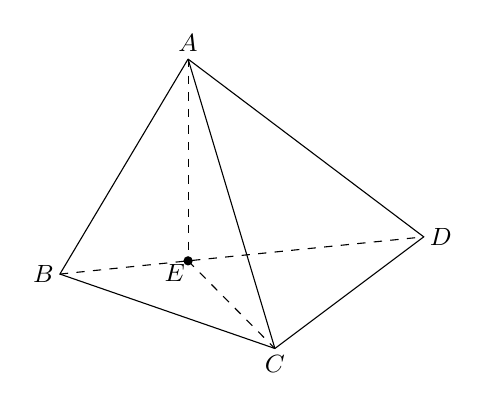
\begin{tikzpicture}[scale=1.05, font=\small]
  \coordinate (A) at (1.55,3.50);
  \coordinate (B) at (0,0.90);
  \coordinate (C) at (2.60,0);
  \coordinate (D) at (4.40,1.35);
  \coordinate (E) at (1.55,1.06);
  % 可见实线
  \draw (A) -- (B) -- (C) -- (D) -- (A);
  \draw (A) -- (C);
  % 被遮挡
  \draw[dashed] (B) -- (E) -- (D);
  \draw[dashed] (A) -- (E);
  \draw[dashed] (E) -- (C);
  \fill (E) circle (1.6pt);
  \node[above,      inner sep=2.5pt] at (A) {$A$};
  \node[left,       inner sep=2pt]   at (B) {$B$};
  \node[below,      inner sep=2.5pt] at (C) {$C$};
  \node[right,      inner sep=2pt]   at (D) {$D$};
  \node[below left, inner sep=1pt]   at (E) {$E$};
\end{tikzpicture}
\end{center}

  (1) 求证：$CD\perp AB$；

  (2) 若 $DE=2$，$BE=1$，$AE=\sqrt{2}$，$CD=2\sqrt{3}$．求直线 $AD$ 与平面 $ABC$ 所成角的正弦值．

\par\medskip

\textbf{(1) 证明}

\textbf{第一步，先证 $AE\perp$ 平面 $BCD$。}

因为 $E$ 在 $BD$ 上，所以 $E\in$ 平面 $BCD$，从而 $CE$、$DE$ 都在平面 $BCD$ 内；又 $C$ 不在直线 $BD$ 上，故 $CE$ 与 $DE$ 是平面 $BCD$ 内的\textbf{两条相交直线}（交点为 $E$）。

已知 $AE\perp CE$，$AE\perp DE$，由\textbf{线面垂直的判定定理}得
\[AE\perp\text{平面 }BCD\]

\textbf{第二步，由此得 $AE\perp CD$。}

因为 $CD\subset$ 平面 $BCD$，由线面垂直的性质
\[AE\perp CD\]

\textbf{第三步，证 $CD\perp$ 平面 $ABD$。}

注意 $E$ 在 $BD$ 上，故 $A$、$D$、$E$ 三点确定的平面\textbf{就是}平面 $ABD$（它同时包含 $B$）。

在平面 $ABD$ 内，$AE$ 与 $AD$ 相交于点 $A$；而已知
\[CD\perp AE\ (\text{第二步}),\qquad CD\perp AD\ (\text{题设})\]

由线面垂直的判定定理
\[CD\perp\text{平面 }ABD\]

\textbf{第四步，收网。} 因为 $AB\subset$ 平面 $ABD$，由线面垂直的性质得
\[CD\perp AB\qquad\blacksquare\]

\begin{gktip}
\textbf{书写红线}：第一步与第三步都用判定定理，两次都必须写全「两条\textbf{相交}直线」及「交点」。第三步还有一个容易被跳过的说明——\textbf{平面 $ADE$ 就是平面 $ABD$}（因为 $E\in BD$），不写这句，后面「$AB\subset$ 平面」就没有依据。
\end{gktip}

\par\medskip

\textbf{(2) 解}

\textbf{建系依据}：由 (1) 已知 $AE\perp$ 平面 $BCD$，取 $EA$ 为 $z$ 轴；$B$、$E$、$D$ 共线，取该直线为 $x$ 轴；由 (1) 的结论 $CD\perp$ 平面 $ABD$ 可得 $CD\perp BD$，故 $DC$ 与 $x$ 轴垂直，取 $DC$ 方向为 $y$ 轴。三轴两两垂直，建系合法。

以 $E$ 为原点。因 $E$ 在\textbf{线段} $BD$ 上，$B$ 与 $D$ 分居 $E$ 两侧，$DE=2$，$BE=1$，$AE=\sqrt2$，$CD=2\sqrt3$：
\[E(0,0,0),\quad D(2,0,0),\quad B(-1,0,0),\quad A\left(0,0,\sqrt2\right),\quad C\left(2,\ 2\sqrt3,\ 0\right)\]

（$C$ 由 $D$ 沿 $y$ 方向平移 $CD=2\sqrt3$ 得到。）

\textbf{条件复核}：$\overrightarrow{EA}\cdot\overrightarrow{EC}=0$ ，$\overrightarrow{EA}\cdot\overrightarrow{ED}=0$ ，$\overrightarrow{DC}\cdot\overrightarrow{DA}=\left(0,2\sqrt3,0\right)\cdot\left(-2,0,\sqrt2\right)=0$ 。四个已知长度也全部吻合。

\textbf{求平面 $ABC$ 的法向量}：
\[\overrightarrow{AB}=\left(-1,0,-\sqrt2\right),\qquad \overrightarrow{AC}=\left(2,2\sqrt3,-\sqrt2\right)\]
\[\vec n=\overrightarrow{AB}\times\overrightarrow{AC}=\begin{vmatrix}\vec i&\vec j&\vec k\\-1&0&-\sqrt2\\2&2\sqrt3&-\sqrt2\end{vmatrix}=\left(2\sqrt6,\ -3\sqrt2,\ -2\sqrt3\right)\]

逐项核对：
\[n_x=0\times\left(-\sqrt2\right)-\left(-\sqrt2\right)\times2\sqrt3=2\sqrt6\]
\[n_y=\left(-\sqrt2\right)\times2-\left(-1\right)\times\left(-\sqrt2\right)=-2\sqrt2-\sqrt2=-3\sqrt2\]
\[n_z=\left(-1\right)\times2\sqrt3-0\times2=-2\sqrt3\]
\[\left|\vec n\right|=\sqrt{24+18+12}=\sqrt{54}=3\sqrt6\]

\textbf{求线面角}：
\[\overrightarrow{AD}=\left(2,0,-\sqrt2\right),\qquad \left|\overrightarrow{AD}\right|=\sqrt{4+2}=\sqrt6\]
\[\vec n\cdot\overrightarrow{AD}=2\sqrt6\times2+\left(-3\sqrt2\right)\times0+\left(-2\sqrt3\right)\times\left(-\sqrt2\right)=4\sqrt6+2\sqrt6=6\sqrt6\]

设所成角为 $\theta$，由线面角公式（用\textbf{正弦}）：
\[\sin\theta=\frac{\left|\vec n\cdot\overrightarrow{AD}\right|}{\left|\vec n\right|\left|\overrightarrow{AD}\right|}=\frac{6\sqrt6}{3\sqrt6\times\sqrt6}=\frac{6\sqrt6}{18}=\frac{\sqrt6}{3}\]

\textbf{所以直线 $AD$ 与平面 $ABC$ 所成角的正弦值为 $\dfrac{\sqrt6}{3}$。}

\begin{gktip}
\textbf{独立验算（等体积法）}：$CD\perp BD$，故
\[S_{\triangle BCD}=\frac12\cdot BD\cdot CD=\frac12\times3\times2\sqrt3=3\sqrt3,\qquad V_{A\text{-}BCD}=\frac13\times3\sqrt3\times\sqrt2=\sqrt6\]
又 $S_{\triangle ABC}=\dfrac12\left|\vec n\right|=\dfrac{3\sqrt6}{2}$，由同一个四面体换底：
\[d(D,\ \text{平面 }ABC)=\frac{3V}{S_{\triangle ABC}}=\frac{3\sqrt6}{\frac{3\sqrt6}{2}}=2\]
\[\sin\theta=\frac{d}{AD}=\frac{2}{\sqrt6}=\frac{\sqrt6}{3}\quad\checkmark\]
两种方法完全独立，结果一致。

\textbf{易错点}：线面角公式用的是 $\sin$（法向量与直线夹角的余弦 = 线面角的正弦），写成 $\cos$ 是本题最常见的整段丢分。
\end{gktip}

\par\medskip

\gksolhead{17}{15 分}

\textbf{题目}　在 $\triangle ABC$ 中，已知 $\cos B=\dfrac{3}{4}$，$\cos^2(A+C)+\sin A\sin C=1$．

  (1) 证明：$\triangle ABC$ 为钝角三角形；

  (2) 若 $\triangle ABC$ 的面积为 $\dfrac{\sqrt{7}}{4}$，求 $\triangle ABC$ 的周长．

\par\medskip

\textbf{(1) 证明}

\textbf{第一步，把 $A+C$ 换成 $B$。} 在三角形中 $A+B+C=\pi$，故 $A+C=\pi-B$：
\[\cos(A+C)=\cos(\pi-B)=-\cos B=-\frac34\]

代入题设条件：
\[\left(-\frac34\right)^2+\sin A\sin C=1\ \Longrightarrow\ \sin A\sin C=1-\frac{9}{16}=\frac{7}{16}\qquad(1)\]

\textbf{第二步，展开 $\cos(A+C)$ 求 $\cos A\cos C$。}
\[\cos(A+C)=\cos A\cos C-\sin A\sin C=-\frac34\]

代入 $(1)$：
\[\cos A\cos C=-\frac34+\frac{7}{16}=-\frac{12}{16}+\frac{7}{16}=-\frac{5}{16}<0\qquad(2)\]

\textbf{第三步，判断。} 因 $A$、$C\in(0,\pi)$，$\cos A$ 与 $\cos C$ 的乘积为负，说明二者\textbf{异号}，即 $A$、$C$ 中\textbf{恰有一个是钝角}（另一个为锐角）。

又 $\cos B=\dfrac34>0$，$B$ 为锐角。

所以 $\triangle ABC$ 有且仅有一个内角为钝角，即 $\triangle ABC$ 为\textbf{钝角三角形}。$\blacksquare$

\begin{gktip}
\textbf{书写红线}：只说「$\cos A\cos C<0$」还不够，必须点明「因此 $A$、$C$ 中恰有一个钝角」，并补一句 $B$ 为锐角，结论才完整。
\end{gktip}

\par\medskip

\textbf{(2) 解}

记 $a=BC$、$b=CA$、$c=AB$（对边记号）。

\textbf{第一步，由面积求 $ac$。} 由 $\cos B=\dfrac34$ 且 $B$ 为锐角：
\[\sin B=\sqrt{1-\frac{9}{16}}=\frac{\sqrt7}{4}\]

\[S=\frac12ac\sin B=\frac12ac\cdot\frac{\sqrt7}{4}=\frac{\sqrt7}{8}ac=\frac{\sqrt7}{4}\ \Longrightarrow\ ac=2\]

\textbf{第二步，由 $(1)$ 求 $b$。} 由正弦定理 $\sin A=\dfrac{a\sin B}{b}$，$\sin C=\dfrac{c\sin B}{b}$，代入第 (1) 问所得 $\sin A\sin C=\dfrac{7}{16}$：
\[\frac{ac\sin^2B}{b^2}=\frac{7}{16}\ \Longrightarrow\ \frac{2\times\frac{7}{16}}{b^2}=\frac{7}{16}\ \Longrightarrow\ b^2=2\ \Longrightarrow\ b=\sqrt2\]

\textbf{第三步，由余弦定理求 $a+c$。}
\[b^2=a^2+c^2-2ac\cos B\ \Longrightarrow\ 2=a^2+c^2-2\times2\times\frac34=a^2+c^2-3\]
\[\Longrightarrow\ a^2+c^2=5\]

于是
\[(a+c)^2=a^2+c^2+2ac=5+2\times2=9\ \Longrightarrow\ a+c=3\quad(\text{取正根})\]

\textbf{第四步，周长。}
\[L=a+b+c=3+\sqrt2\]

\textbf{所以 $\triangle ABC$ 的周长为 $3+\sqrt2$。}

\begin{gktip}
\textbf{验算（还原三边）}：$a+c=3$、$ac=2$，故 $a$、$c$ 是 $t^2-3t+2=0$ 的两根，即 $\{a,c\}=\{1,2\}$。三边为 $1$、$2$、$\sqrt2$：
\begin{itemize}
\item 检查 $\cos B$：$b=\sqrt2$ 所对，$\dfrac{1^2+2^2-2}{2\times1\times2}=\dfrac34$ 
\item 检查面积：$\dfrac12\times1\times2\times\dfrac{\sqrt7}{4}=\dfrac{\sqrt7}{4}$ 
\item 检查钝角：最大边 $2$ 所对角的余弦 $=\dfrac{1+2-4}{2\times1\times\sqrt2}=-\dfrac{\sqrt2}{4}<0$，确为钝角  与第 (1) 问一致。
\end{itemize}

\textbf{方法总结}：第 (2) 问的关键是\textbf{别急着解 $a$、$c$}。先用面积拿 $ac$、用正弦定理拿 $b$、用余弦定理拿 $a^2+c^2$，最后靠 $(a+c)^2=a^2+c^2+2ac$ 一步得到周长——全程不需要知道 $a$、$c$ 各是多少。
\end{gktip}

\par\medskip

\gksolhead{18}{17 分}

\textbf{题目}　椭圆 $E$：$\dfrac{x^2}{a^2}+y^2=1$（$a>1$），过右焦点且与 $x$ 轴垂直的直线被 $E$ 截得的长度为 $\sqrt{2}$．

  (1) 求 $E$ 的离心率．

  (2) $O$ 为坐标原点，给定点 $G(t_0,0)$（$t_0\ne0$），$A(x_0,y_0)$（$y_0\ne0$）在 $E$ 上，过点 $A$ 作 $y$ 轴的垂线，垂足为 $B$，$AO$ 与 $GB$ 交于点 $P$．当 $A$ 在 $E$ 上运动时，$P$ 的轨迹为 $M$．

  　（ⅰ）求 $M$ 的方程，并说明 $M$ 是什么曲线；

  　（ⅱ）$M$ 是否有中心点？当 $t_0$ 为何值时，$M$ 有中心点？当 $M$ 有中心点时，平移 $M$ 到 $M'$，使 $O$ 为 $M'$ 的中心点，说明 $M'$ 的形状．

\par\medskip

\textbf{(1) 解}

题中 $b^2=1$，即 $b=1$。「过焦点且垂直于长轴的弦」就是\textbf{通径}，长度公式为 $\dfrac{2b^2}{a}$：
\[\frac{2\times1}{a}=\sqrt2\ \Longrightarrow\ a=\frac{2}{\sqrt2}=\sqrt2\]

满足 $a>1$ 。于是
\[a^2=2,\quad b^2=1,\quad c^2=a^2-b^2=1,\quad c=1\]

\[e=\frac{c}{a}=\frac{1}{\sqrt2}=\frac{\sqrt2}{2}\]

\textbf{所以 $E$ 的离心率为 $\dfrac{\sqrt2}{2}$，且 $E:\dfrac{x^2}{2}+y^2=1$。}

\par\medskip

\textbf{(2)（ⅰ）解}

\textbf{第一步，写出两条直线并求交点。}

$A(x_0,y_0)$ 在 $E$ 上且 $y_0\ne0$；过 $A$ 作 $y$ 轴的垂线，垂足为
\[B(0,y_0)\]

\begin{itemize}
\item 直线 $AO$：过原点与 $A$，其上的点可写成 $\left(\lambda x_0,\ \lambda y_0\right)$（$\lambda\in\mathbb{R}$）；
\item 直线 $GB$：过 $G(t_0,0)$ 与 $B(0,y_0)$，两个截距均非零，用\textbf{截距式}最省事：
\end{itemize}
\[\frac{x}{t_0}+\frac{y}{y_0}=1\]

把 $AO$ 上的点代入 $GB$：
\[\frac{\lambda x_0}{t_0}+\frac{\lambda y_0}{y_0}=1\ \Longrightarrow\ \lambda\left(\frac{x_0}{t_0}+1\right)=1\ \Longrightarrow\ \lambda=\frac{t_0}{x_0+t_0}\]

（这里需 $x_0+t_0\ne0$，否则 $AO\parallel GB$，交点 $P$ 不存在。）

于是
\[P:\quad x=\frac{t_0x_0}{x_0+t_0},\qquad y=\frac{t_0y_0}{x_0+t_0}\qquad(\bigstar)\]

\textbf{第二步，反解出 $x_0$、$y_0$（消参的标准做法）。}

由 $(\bigstar)$ 的第一式，$x\left(x_0+t_0\right)=t_0x_0$，整理得
\[x_0\left(x-t_0\right)=-t_0x\ \Longrightarrow\ x_0=\frac{t_0x}{t_0-x}\]

进而
\[x_0+t_0=\frac{t_0x+t_0\left(t_0-x\right)}{t_0-x}=\frac{t_0^2}{t_0-x}\]

代入 $(\bigstar)$ 的第二式：
\[y=\frac{t_0y_0\left(t_0-x\right)}{t_0^2}\ \Longrightarrow\ y_0=\frac{t_0y}{t_0-x}\]

\textbf{第三步，代入椭圆方程消参。} 把上两式代入 $\dfrac{x_0^2}{2}+y_0^2=1$：
\[\frac{t_0^2x^2}{2\left(t_0-x\right)^2}+\frac{t_0^2y^2}{\left(t_0-x\right)^2}=1\]

两边同乘 $\left(t_0-x\right)^2$：
\[t_0^2\left(\frac{x^2}{2}+y^2\right)=\left(t_0-x\right)^2=t_0^2-2t_0x+x^2\]

移项整理，得 $M$ 的方程：
\[\boxed{\left(\frac{t_0^2}{2}-1\right)x^2+t_0^2y^2+2t_0x-t_0^2=0\qquad(y\ne0)}\]

（其中 $y\ne0$ 来自题设 $y_0\ne0$。）

\textbf{第四步，判断曲线类型。} 记
\[\lambda=\frac{t_0^2}{2}-1=\frac{t_0^2-2}{2}\]

$x^2$ 项系数为 $\lambda$，$y^2$ 项系数为 $t_0^2>0$，无 $xy$ 项，故按 $\lambda$ 的符号分三类：

\begin{itemize}
\item \textbf{当 $\left|t_0\right|>\sqrt2$ 时}，$\lambda>0$，两个平方项系数同号。配方（见下问）后右端为正，$M$ 是\textbf{椭圆}。
\end{itemize}
  又若为圆需 $\lambda=t_0^2$，即 $\dfrac{t_0^2-2}{2}=t_0^2$，得 $t_0^2=-2$，不可能，故\textbf{不会退化为圆}。
\begin{itemize}
\item \textbf{当 $\left|t_0\right|=\sqrt2$ 时}，$\lambda=0$，方程化为 $2y^2+2t_0x-t_0^2=0$，即
\end{itemize}
\[y^2=1-t_0x\]
  $M$ 是\textbf{抛物线}（开口方向由 $t_0$ 的符号决定）。
\begin{itemize}
\item \textbf{当 $0<\left|t_0\right|<\sqrt2$ 时}，$\lambda<0$，两个平方项系数异号，$M$ 是\textbf{双曲线}。
\end{itemize}

\textbf{补充说明（去点）}：由 $y_0\ne0$ 知 $y\ne0$，即上述二次曲线上位于 $x$ 轴的点要\textbf{去掉}——它们恰是 $A$ 取到椭圆左右顶点 $\left(\pm\sqrt2,0\right)$ 时的像。

\begin{gktip}
\textbf{几何解释}：$(\bigstar)$ 表明 $P$ 是 $A$ 在「以 $\left(-t_0,0\right)$ 所在竖直线为消失线」的中心投影下的像。当 $\left|t_0\right|>\sqrt2$ 时直线 $x_0=-t_0$ 与椭圆\textbf{不相交}，像是有界的 → 椭圆；相切（$\left|t_0\right|=\sqrt2$）→ 抛物线；相交于两点（$\left|t_0\right|<\sqrt2$）→ 双曲线（那两点被送到无穷远，成为渐近方向）。这解释了三类曲线为何恰以 $\left|t_0\right|=\sqrt2$ 分界。
\end{gktip}

\par\medskip

\textbf{(2)（ⅱ）解}

\textbf{第一问：$M$ 何时有中心点。}

「中心点」即曲线的\textbf{对称中心}。上一问的分类给出：
\begin{itemize}
\item $\left|t_0\right|=\sqrt2$ 时 $M$ 为抛物线，\textbf{没有}对称中心；
\item $\left|t_0\right|\ne\sqrt2$（且 $t_0\ne0$）时 $M$ 为椭圆或双曲线，\textbf{有}对称中心。
\end{itemize}

\textbf{所以：当且仅当 $t_0\ne\pm\sqrt2$（题设已有 $t_0\ne0$）时，$M$ 有中心点。}

\textbf{第二问：求中心并平移。}

设 $\lambda=\dfrac{t_0^2-2}{2}\ne0$，对 $M$ 的方程按 $x$ 配方：
\[\lambda x^2+2t_0x=\lambda\left(x+\frac{t_0}{\lambda}\right)^2-\frac{t_0^2}{\lambda}\]

于是 $M$ 化为
\[\lambda\left(x+\frac{t_0}{\lambda}\right)^2+t_0^2y^2=t_0^2+\frac{t_0^2}{\lambda}=t_0^2\cdot\frac{\lambda+1}{\lambda}=t_0^2\cdot\frac{\frac{t_0^2}{2}}{\lambda}=\frac{t_0^4}{2\lambda}\]

可见 $M$ 的中心点为
\[\left(-\frac{t_0}{\lambda},\ 0\right)=\left(-\frac{2t_0}{t_0^2-2},\ 0\right)\]

把 $M$ 沿 $x$ 轴平移 $\dfrac{t_0}{\lambda}$ 个单位（即令 $X=x+\dfrac{t_0}{\lambda}$，$Y=y$），得以 $O$ 为中心的 $M'$：
\[\lambda X^2+t_0^2Y^2=\frac{t_0^4}{2\lambda}\]

两边同除右端，并代入 $2\lambda=t_0^2-2$，得 $M'$ 的标准形式：
\[\boxed{\frac{X^2}{\dfrac{2t_0^4}{\left(t_0^2-2\right)^2}}+\frac{Y^2}{\dfrac{t_0^2}{t_0^2-2}}=1}\]

\textbf{第三问：$M'$ 的形状。}

记 $A^2=\dfrac{2t_0^4}{\left(t_0^2-2\right)^2}>0$，$B^2=\dfrac{t_0^2}{t_0^2-2}$。

\begin{itemize}
\item \textbf{当 $\left|t_0\right|>\sqrt2$ 时}：$B^2>0$，$M'$ 是\textbf{中心在原点、焦点在 $x$ 轴上的椭圆}。
\end{itemize}
  理由（比较长短轴）：
\[\frac{A^2}{B^2}=\frac{2t_0^4}{\left(t_0^2-2\right)^2}\cdot\frac{t_0^2-2}{t_0^2}=\frac{2t_0^2}{t_0^2-2}>2>1\]
  故 $A>B$，长轴在 $x$ 轴上；且如 (ⅰ) 所证 $A\ne B$，不会是圆。
\begin{itemize}
\item \textbf{当 $0<\left|t_0\right|<\sqrt2$ 时}：$B^2<0$，把方程改写为
\end{itemize}
\[\frac{X^2}{\dfrac{2t_0^4}{\left(2-t_0^2\right)^2}}-\frac{Y^2}{\dfrac{t_0^2}{2-t_0^2}}=1\]
  $M'$ 是\textbf{中心在原点、实轴在 $x$ 轴上（焦点在 $x$ 轴上）的双曲线}。

（两种情形下 $M'$ 同样要去掉它与 $x$ 轴的两个交点；这两点关于 $O$ 对称，不影响 $O$ 是中心点。）

\begin{gktip}
\textbf{具体例子（自检用）}
\begin{itemize}
\item 取 $t_0=2$：$\lambda=1$，$M:\ x^2+4y^2+4x-4=0$，即 $\dfrac{(x+2)^2}{8}+\dfrac{y^2}{2}=1$，中心 $(-2,0)$，$M':\dfrac{X^2}{8}+\dfrac{Y^2}{2}=1$ 为椭圆。代公式：$A^2=\dfrac{2\times16}{4}=8$ ，$B^2=\dfrac{4}{2}=2$ 。
\item 取 $t_0=1$：$\lambda=-\dfrac12$，$M:\ -\dfrac12x^2+y^2+2x-1=0$，即 $\dfrac{(x-2)^2}{2}-y^2=1$，中心 $(2,0)$，$M':\dfrac{X^2}{2}-Y^2=1$ 为双曲线。代公式：$A^2=\dfrac{2\times1}{1}=2$ ，$B^2=\dfrac{1}{-1}=-1$ 。
\end{itemize}

\textbf{方法总结}：轨迹题的通用流程是「\textbf{设动点 → 用参数表示 → 反解参数 → 代入已知曲线}」。本题的两个关卡是：① 反解 $x_0$、$y_0$ 时不要漏掉 $x_0+t_0\ne0$；② 分类讨论的分界点由 $x^2$ 项系数 $\lambda$ 的符号决定，$\lambda=0$（即 $\left|t_0\right|=\sqrt2$）恰是「有心 / 无心」的分水岭，这正是第（ⅱ）问要问的东西。
\end{gktip}

\par\medskip

\gksolhead{19}{17 分}

\textbf{题目}　已知函数 $f(x)=x\mathrm{e}^x+ax+b$，曲线 $y=f(x)$ 在点 $\left(0,f(0)\right)$ 处的切线为 $y=-2x+1$．

  (1) 求 $a$，$b$；

  (2) 当 $x>0$ 时，$f(x+m)-f(x)>m$，求 $m$ 的取值范围；

  (3) 当 $x>0$ 时，$f(x+k)+f(k-x)>2f(k)$，求 $k$ 的最小值．

\par\medskip

\textbf{(1) 解}

切线给出\textbf{两个}信息：切点纵坐标与斜率。

\textbf{切点}：$f(0)=0\cdot\mathrm e^0+0+b=b$；切线在 $x=0$ 处的值为 $-2\times0+1=1$。故
\[b=1\]

\textbf{斜率}：
\[f'(x)=\mathrm e^x+x\mathrm e^x+a=(x+1)\mathrm e^x+a\]
\[f'(0)=1+a=-2\ \Longrightarrow\ a=-3\]

\[\boxed{a=-3,\quad b=1}\]

即
\[f(x)=x\mathrm e^x-3x+1\]

\par\medskip

\textbf{(2) 解}

\textbf{第一步，剥离线性部分。} 记
\[g(t)=t\mathrm e^{t}\]

则 $f(t)=g(t)-3t+1$，于是
\[f(x+m)-f(x)=g(x+m)-g(x)-3m\]

原不等式 $f(x+m)-f(x)>m$ 等价于
\[g(x+m)-g(x)>4m\qquad\text{对一切 }x>0\text{ 成立}\qquad(\sharp)\]

\textbf{第二步，讨论 $m$ 的符号。} 令
\[h(x)=g(x+m)-g(x)=(x+m)\mathrm e^{x+m}-x\mathrm e^{x}\]

\textbf{情形一：$m<0$。} 提出 $\mathrm e^x$：
\[h(x)=\mathrm e^{x}\left[(x+m)\mathrm e^{m}-x\right]=\mathrm e^{x}\left[x\left(\mathrm e^{m}-1\right)+m\mathrm e^{m}\right]\]

因 $m<0$ 时 $\mathrm e^m<1$，方括号是关于 $x$ 的\textbf{递减}一次式，当 $x\to+\infty$ 时趋于 $-\infty$；再乘以 $\mathrm e^x\to+\infty$，故 $h(x)\to-\infty$。必存在 $x>0$ 使 $h(x)<4m$，$(\sharp)$ 不成立。\textbf{舍去。}

\textbf{情形二：$m=0$。} 此时 $h(x)\equiv0$，$4m=0$，不等式成为 $0>0$，不成立。\textbf{舍去。}

\textbf{情形三：$m>0$。} 求导：
\[h'(x)=g'(x+m)-g'(x)=(x+m+1)\mathrm e^{x+m}-(x+1)\mathrm e^{x}=\mathrm e^{x}\left[(x+m+1)\mathrm e^{m}-(x+1)\right]\]

因 $m>0$ 时 $\mathrm e^m>1$ 且 $x+m+1>x+1>0$，得
\[(x+m+1)\mathrm e^{m}-(x+1)>(x+m+1)-(x+1)=m>0\]

故 $h'(x)>0$，$h$ 在 $[0,+\infty)$ 上\textbf{严格递增}。于是对一切 $x>0$：
\[h(x)>h(0)=g(m)-g(0)=m\mathrm e^{m}\]

且 $h(0)=m\mathrm e^m$ 是 $h$ 在 $(0,+\infty)$ 上的\textbf{下确界}（取不到）。因此
\[(\sharp)\ \text{成立}\iff m\mathrm e^{m}\ge 4m\overset{m>0}{\iff}\mathrm e^{m}\ge4\iff m\ge\ln4=2\ln2\]

\begin{itemize}
\item 若 $m\ge2\ln2$：对一切 $x>0$ 有 $h(x)>m\mathrm e^m\ge4m$ （注意 $h(x)>h(0)$ 是\textbf{严格}的，故 $m=2\ln2$ 时等号不会真的取到，不等式仍严格成立）。
\item 若 $0<m<2\ln2$：$h(0)=m\mathrm e^m<4m$，由 $h$ 连续，存在充分小的 $x>0$ 使 $h(x)<4m$ 。
\end{itemize}

\[\boxed{m\ \text{的取值范围是}\ \left[2\ln2,\ +\infty\right)}\]

\begin{gktip}
\textbf{临界点核验}：$m=2\ln2$ 时 $\mathrm e^m=4$，$m\mathrm e^m=8\ln2\approx5.545$，$4m=8\ln2\approx5.545$，二者\textbf{恰好相等}——这正是「下确界取不到」保证了不等式仍严格成立的临界情形。
\end{gktip}

\par\medskip

\textbf{(3) 解}

\textbf{第一步，线性项完全抵消。} 仍记 $g(t)=t\mathrm e^t$，$f(t)=g(t)-3t+1$。计算线性与常数部分：
\[\left[-3(x+k)+1\right]+\left[-3(k-x)+1\right]-2\left[-3k+1\right]=-3x-3k+1-3k+3x+1+6k-2=0\]

故原不等式等价于
\[\varphi(x):=\mathrm e^{-k}\left[g(k+x)+g(k-x)-2g(k)\right]>0\qquad\text{对一切 }x>0\text{ 成立}\]

\textbf{第二步，把 $\varphi$ 写成便于求导的形式。}
\[g(k+x)+g(k-x)-2g(k)=(k+x)\mathrm e^{k+x}+(k-x)\mathrm e^{k-x}-2k\mathrm e^{k}\]
\[=\mathrm e^{k}\left[(k+x)\mathrm e^{x}+(k-x)\mathrm e^{-x}-2k\right]\]

所以
\[\varphi(x)=k\left(\mathrm e^{x}+\mathrm e^{-x}-2\right)+x\left(\mathrm e^{x}-\mathrm e^{-x}\right)\]

（把含 $k$ 的项与含 $x$ 的项分开，是本题的关键整理。）

\textbf{第三步，两次求导，把 $k$ 逼出来。}
\[\varphi(0)=0\]
\[\varphi'(x)=k\left(\mathrm e^{x}-\mathrm e^{-x}\right)+\left(\mathrm e^{x}-\mathrm e^{-x}\right)+x\left(\mathrm e^{x}+\mathrm e^{-x}\right),\qquad \varphi'(0)=0\]
\[\varphi''(x)=k\left(\mathrm e^{x}+\mathrm e^{-x}\right)+2\left(\mathrm e^{x}+\mathrm e^{-x}\right)+x\left(\mathrm e^{x}-\mathrm e^{-x}\right)\]
\[\boxed{\varphi''(x)=(k+2)\left(\mathrm e^{x}+\mathrm e^{-x}\right)+x\left(\mathrm e^{x}-\mathrm e^{-x}\right)}\]

注意当 $x>0$ 时 $\mathrm e^x+\mathrm e^{-x}>0$ 且 $x\left(\mathrm e^x-\mathrm e^{-x}\right)>0$。

\textbf{充分性（$k\ge-2$ 时成立）}：此时 $k+2\ge0$，故对一切 $x>0$
\[\varphi''(x)\ge0+x\left(\mathrm e^{x}-\mathrm e^{-x}\right)>0\]

于是 $\varphi'$ 在 $[0,+\infty)$ 严格递增，$\varphi'(x)>\varphi'(0)=0$；进而 $\varphi$ 严格递增，$\varphi(x)>\varphi(0)=0$ 。

\textbf{必要性（$k<-2$ 时不成立）}：此时
\[\varphi''(0)=(k+2)\times2+0=2(k+2)<0\]

由 $\varphi''$ 连续，存在 $\delta>0$ 使 $\varphi''(x)<0$ 在 $[0,\delta)$ 上成立。于是 $\varphi'$ 在 $[0,\delta)$ 递减，$\varphi'(x)<\varphi'(0)=0$；进而 $\varphi$ 在 $[0,\delta)$ 递减，$\varphi(x)<\varphi(0)=0$ ，不等式不成立。

\textbf{第四步，结论。} 条件成立当且仅当 $k\ge-2$，故

\[\boxed{k\ \text{的最小值为}\ -2}\]

\begin{gktip}
\textbf{临界点核验（$k=-2$）}：此时 $\varphi(x)=x\left(\mathrm e^x-\mathrm e^{-x}\right)-2\left(\mathrm e^x+\mathrm e^{-x}-2\right)$。展开成幂级数可见首项为 $\dfrac{x^4}{6}$，确为正；数值上 $\varphi(0.1)\approx1.667\times10^{-5}>0$、$\varphi(1)\approx0.178>0$，与结论一致。

\textbf{背后的几何意义}：条件 $\dfrac{g(k+x)+g(k-x)}{2}>g(k)$ 说的是「$g$ 在 $k$ 处\textbf{严格中点凸}」。而
\[g''(t)=(t+2)\mathrm e^{t}\]
的零点恰为 $t=-2$——$g$ 在 $(-\infty,-2)$ 上凹、在 $(-2,+\infty)$ 上凸，$t=-2$ 是\textbf{拐点}。答案 $k_{\min}=-2$ 正是这个拐点：在拐点及其右侧，中点凸性仍严格成立（拐点处二阶导为零但四阶效应仍为正）；一旦落到拐点左侧，局部凹性立刻破坏不等式。

\textbf{方法总结}：第 (2)、(3) 问共用同一套招式——\textbf{先把 $f$ 中的线性项剥掉，只留 $g(t)=t\mathrm e^t$}（(2) 中线性项贡献 $-3m$ 并入常数，(3) 中线性项完全抵消）。随后 (2) 靠一阶导判单调、比下确界，(3) 靠二阶导在 $x=0$ 处的符号判局部凹凸。凡「对一切 $x>0$ 恒成立、且 $x\to0^+$ 时两边相等」的题型，都应优先考察端点处的各阶导数符号。
\end{gktip}
